Avsnitt~\ref{sec:run-amba} beskriver hur AMBA installeras och körs. Detta
avsnitt diskuterar utvalda delar av AMBAs implementationsdetaljer.

AMBA ska betraktas som ett system bestående av en huvudprocess och en
bakgrundsprocess. Huvudprocessen är ett grafiskt Rust-program bestående av flera
beständiga trådar som kommunicerar med varandra genom delat minne och
meddelanden. Bakgrundsprocessen är en \stoe{}-instans startad av huvudprocessen
med \stoe{}-pluginet AmbaPlugin som möjliggör kommunikation mellan
huvudprocessen och \stoe{} självt. IPC mellan huvudprocessen och
bakgrundsprocessen sker över två Unix-socketar. Figur~\ref{fig:arkitektur} visar
en översikt av AMBAs arkitektur.

\begin{figure}[h]
    \centering
    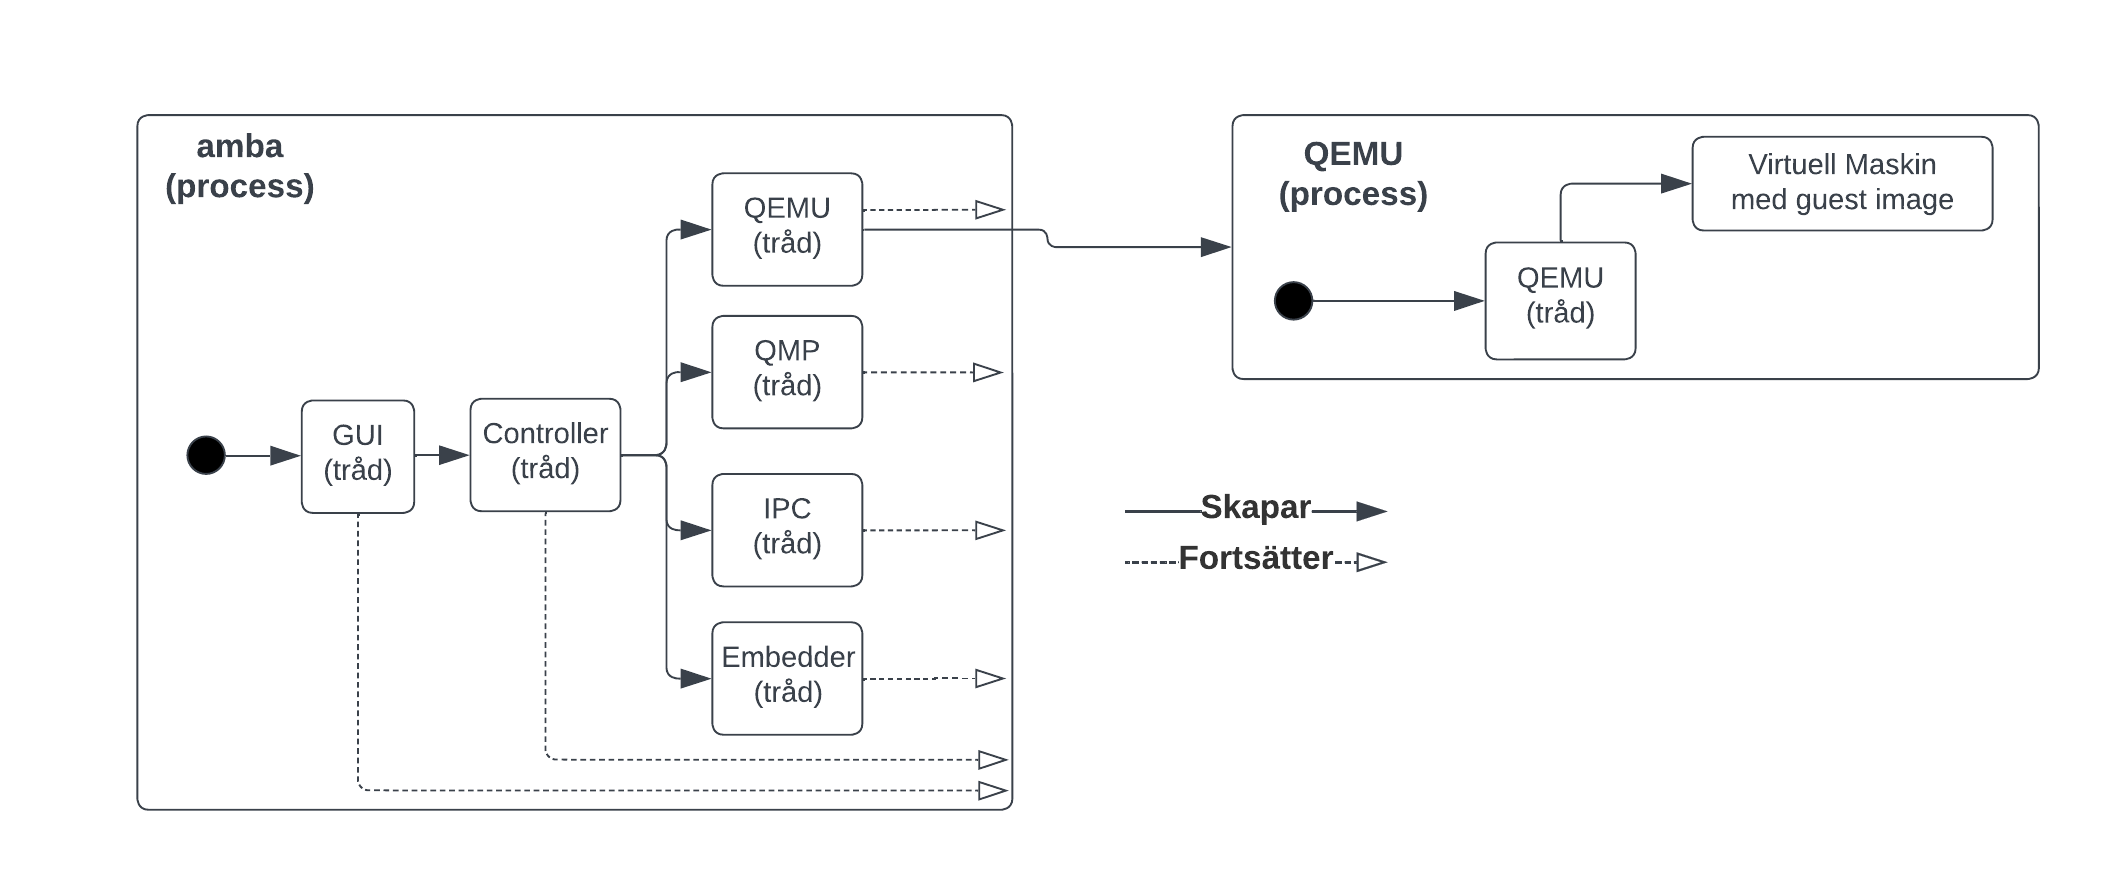
\includegraphics[width=\textwidth]{figures/arch-process-threads.png}
    \caption{AMBA: skapande av processer och trådar}\label{fig:arkitektur}
\end{figure}

\begin{figure}[h]
    \centering
    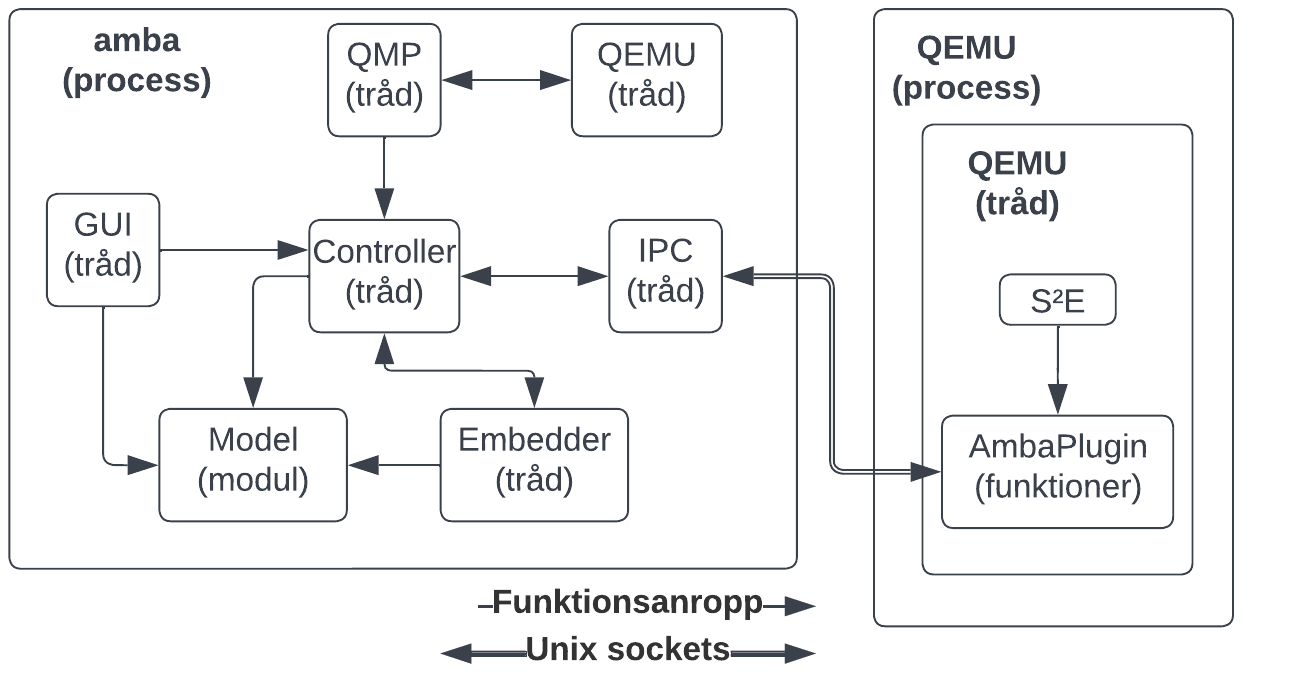
\includegraphics[width=\textwidth]{figures/arch-communication.png}
    \caption{AMBA: kommunikation mellan processer och trådar}\label{fig:arkitektur-kommunikation}
\end{figure}


\section{Huvudprocess}

Huvudprocessen kör 6 beständiga trådar.
Huvudtråden eller GUI-tråden, som äger och hanterar det grafiska gränssnittet.
Kontrolltråden (controller), som är mellanhand i all meddelandebaserad
kommunikation mellan trådar och även är avsändare för IPC till AmbaPlugin.
Utplaceringstråden (embedder), som tar emot instruktioner från kontrolltråden,
kör den beräkningsmässigt tunga nodutplaceringen på de fem graferna och skriver
denna till minne tillgängligt från GUI-tråden.
IPC-tråden, som tar emot meddelanden över IPC från AmbaPlugin.
QMP-tråden, som tar emot och skickar meddelanden till QEMU.\@ QMP står för QEMU
Machine Protocol och möjliggör programmatisk kontroll av QEMU-instansen direkt.
QMP-tråden har en väldigt begränsad funktion och är inte nödvändig för AMBAs
nuvarande funktionalitet.
QEMU-tråden, som startar QEMU/\stoe{}-instansen och inväntar dess avslutande.
Detta inväntande är bland annat nödvändigt för att hantera en krasch i \stoe{}
eller AmbaPlugin på ett bra sätt.

\subsection{Uppstart}

Som beskrivet i avsnitt~\ref{sec:run-amba} startas AMBA av användaren med en
angiven receptfil. Huvudprocessen tolkar receptfilen och genererar den
konfiguration som \stoe{} behöver för att köra den analyserade binären så som
receptfilen specifierat. Huvudprocessen startar alla beständiga trådar och
QEMU-tråden startar QEMU.\@ QEMU startas från en minnesavbild av en virtuell
maskin anpassad till \stoe{}, och en process kallad bootstrap körs som
förbereder den virtuella maskinen inför den symboliska exekveringen. Denna
förberedelse innebär till exempel att \verb|/tmp/| som innehåller de symboliska
filerna placeras i ett RAM-uppbackat tmpfs och att de symboliska filerna görs
symboliska. Binären som ska analyseras skickas in i QEMU, startas och \emph{hooks} till
AmbaPlugin börjar sampla data som ska skickas till huvudprocessen. Datan skickas
till huvudprocessen som börjar visa grafen när den byggs och samtidigt
kontinuerligt utplaceras.

\subsection{GUI}

Huvudprocessen använder immediate-mode-gui-biblioteket egui~\cite{egui} för att
rita sitt gränssnitt. Detta innebär att hela fönstret ritas om varje bildruta,
mer likt typisk spelgrafik än klassiska grafiska gränssnitt. egui är enkelt att
utveckla för vilket var kritiskt för att utveckla prototypen AMBA under detta
kandidatarbete. Grafvykomponenten är byggd från grundläggande egui-komponenter
vilket gjorde bibliotekets utvecklarergonomi viktig.

\section{\stoe{}}\label{sec:s2e}

Den symboliska exekveringsmotorn \stoe{} beskrivs mer översiktligt i
avsnitt~\ref{sec:befintliga-ramverk}. Detta avsnitt diskuterar dess användning
i AMBA och den funktionalitet som är relevant för detta.\@

\stoe{} tillhandahåller en hel virtuell maskin med stöd för symbolisk exekvering
genom att bygga ovanpå på QEMU.\@ \stoe{} är ett dynamisk bibliotek som
\verb|LD_PRELOAD|:as i en modifierad QEMU 3.0.0 och lägger till stöd för
symboliska värden i register och RAM.\@

\stoe{} kan fristående agera som automatisk symbolisk fuzzer och producera
konkret indata motsvarande olika symboliska lövtillstånd. Men \stoe{} är
komplext, har mycket som kan konfigureras och dess fulla kraft är tillgänglig
endast för \stoe{}-plugin~\cite{Chipounov12}.

Plugin har möjlighet att följa \stoe{}:s exekvering genom återanropsfunktioner och
undersöka egenskaper för att spåra och forma analyser. Plugin kan även påverka
den symboliska exekveringen, till exempel genom att i realtid ange vilka
tillstånd som ska exekveras och vilka som ska pausas.

Konceptuellt består ett S2E plugin av ett tillstånd och en initieringsfuktion.
Tillståndet ärvs från ett kärn-plugin som innehåller information om bl.a.\
programtillstånd, symbolisk exekveringstillstånd och information om andra
plugin. Tillståndet kan utökas för att samla information, kontrollera egenskaper
och utföra binäranalys. Initieringsfunktionen består av tillståndsinitiering och
registrering av återanropsfunktioner till olika \emph{hooks} som tillgängligörs av antingen S2E:s
kärn-plugin eller andra plugin. Dessa återanropsfunktioner anropas under exekvering när
motsvarande villkor för en \emph{hook} uppfylls.

AmbaPlugin är ett S2E plugin som har utvecklats för att samla information under
exekvering av en binär ämnat för att visualisera exekveringen i AMBA.\@
AmbaPlugin kan även bestämma ett subträd av tillstånd vars exekvering ska
prioriteras före andra.

\subsection{AmbaPlugin}

AmbaPlugin registrerar återanropsfunktioner för ett antal \emph{hooks}, inklusive bland annat
\texttt{onStateFork}, \texttt{onTranslateBlockComplete} och
\texttt{onBlockStart}. När dessa \emph{hooks} anropas samlas information om S2E:s
tillståndsid, generation för ett block i fallet av självmodifierande kod,
virtuell adress, maskinkod etc.

Utifrån detta framställs kantinformation för kontrollflödesgrafen och
tillståndsgrafen som kontinuerligt skickas över IPC till huvudprocessen. Denna
iterativa informationsuppdateringen är nödvändigt för att uppdatera
användargränssnittet i realtid, alltså flera gånger per sekund. Få verkliga
binärer har tillståndsgrafer som kan konstrueras fullständigt.

\subsection{Paketering i pakethanteraren Nix}

\stoe{} är ett komplicerat system som innehåller bland annat QEMU, Linux, KLEE
och LLVM.\@ Dess bygge var trasigt när vi påbörjade detta kandidatarbete (t.ex.\
felaktiga git-remote-url:er för QEMU-projektet), flera andra småsaker hindrade
byggande och utöver allt detta rekommenderades en Docker-miljö för att hantera
bygget med dess alla beroende komponenter. För att förbättra bygget, uppnå
bättre reproducerbarhet samt bättre samspel med en grafisk applikation paketeras
\stoe{} i Nix.

Nix-paketet \stoe{} har framställts för utveckling av AMBA och är inte lämpligt
för upstreaming till \stoe{} i nuvarande form men detta kan vara möjligt efter
utökningar och modifieringar.

\section{Grafbehandling}

Huvudprocessen tar emot en ström av kanter representerade som ordnade par av
nodmetadata, där mottagandet av en kant innebär att den kanten precis
bevandrats. Olika symboliska tillstånd har olika noder, vilket innebär att denna
kantströmmen innehåller all information som huvudprocessen behöver.

Nya noder placeras i en hashtabell och får ett sekventiellt allokerat id. Detta
id används sedan för att identifiera noden i olika representationer av grafen.
Grafen representeras med en grannlista för linjegrafskompression och nedbrytning
i starkt ansluta komponenter och med en kantlista för nodutplacering genom
kraftsimulation. I båda dessa sammanhang är det praktiskt att noder
representeras som registerstora tal.

\subsection{Linjegrafskompression}

AMBA presenterar både en komprimerad och en okomprimerad graf för användaren.
Grafen komprimeras genom kantkontraktion av alla kanter anslutna till en nod av
ingrad exakt ett och utgrad exakt ett. Detta är ekvivalent med att se alla par
av basic blocks som alltid förekommer efter varandra som ett enda basic block.
Detta ger komprimerade basic blocks som kan spänna flera funktioner och dynamiskt
länkade bibliotek.

Grafkompressionen sker online, alltså genom en datastruktur som samtidigt
tillåter tilläggning av kanter i grafen och kan svara på frågor om vilka kanter
som kommer in samt går ut från en (komprimerad) nod. Detta implementeras genom
att lagra både en komprimerad och okomprimerad graf. En pekare till den
okomprimerade grafen delas ut till läsare. När en kant ska läggas till
kontrolleras först om denna redan finns i den okomprimerade grafen. Om inte
återställs de kantkontraktioner som skapat de komprimerade noder som innehåller
kantens ändnoder. Därefter läggs kanten till och grafen komprimeras lokalt.
Tidskomplexiteten för kanttilläggningar är då lika med summan av kardinaliteten
på de komprimerade noder som innehåller kantens slutnoder. Detta är kvadratiskt
i värstafallet en enda linjegraf men fungerar i praktiken då
kontrollflödesgrafen inte innehåller långa linjegrafer. Författarna är medvetna
om att en fullt linjär algoritm existerar.

\subsection{Starkt anslutna komponenter}

AMBA kan färglägga noder i de komprimerade och ickekomprimerade
kontrollflödesgraferna efter deras så kallade starkt anslutna komponent (jrf.\
eng.\ strongly connected component). En riktad grafs starkt anslutna komponenter
är ekvivalensklasserna under relationen att ett par av noder är både nedströms
och uppströms ifrån varandra. Den starkt anslutna komponenten som en nod $V$
tillhör är alltså mängden av de noder som både kan nå $V$ och som kan nås av
$V$.

AMBA bryter ned grafer i deras starkt anslutna komponenter med Tarjans
algoritm~\cite{tarjan}. Tarjans algoritm bygger på en rekursiv DFS, och AMBA
hanterar dess linjära stackdjup genom att köra algoritmen på en tråd med en
tillräckligt stor stack.

\subsection{Nodutplacering genom kraftsimulation}

Nodutplaceringen styrs av en attraktionskraft mellan kopplade noder som är
proportionelig mot $D^{1.2}$ på avståndet $D$, en repulsionskraft mellan alla
par av noder som är proportionelig mot $\frac{D}{1+D^3}$ och en
gravitationskraft som påverkar alla noder utom rotnoden i negativ y-led.

Hastighet och position integreras med Euler framåt, men magnituden på
hastigheten ändras dessutom direkt: den ökas exponentiellt när accelerationen
och hastigheten är likriktade och minskas exponentiellt annars. Detta ger
snabbare konvergens. Positionen kan även uppdateras med uniformt brus om
användaren har ställt in detta som nollskilt.

Slutligen gäller tvång som placerar rotnoden i origo och masscentrum på axeln
vertikalt under. Därmed går exekvering framförallt uppifrån ned.

Den beräkningstunga delen av nodutplaceringen är beräkningen av
repulsionskraften. Naiv summation mellan varje par av noder tar $O(n^2)$ tid per
tidssteg eller $O(n^3)$ tid totalt under antagande att konvergens nås efter
linjärt många steg. Därför implementerar AMBA även Barnes-Hut
kraftberäkningsalgoritm på ett R-träd. Ett R-träd är ett balanserat binärt träd
av punktmängder där varje lövnod är en enskild punkt och varje grennod lagrar
begränsningslådan för punkterna den innehåller. AMBA bygger trädet genom att
rekursivt hugga den axel som är geometriskt längst och använder en parameter för
att bestämma vid kvot mellan lådstorlek och kraftavstånd där lådan anses
tillräckligt liten för att dess noder kan approximeras ligga i lådans
masscentrum. Barnes-Hut har en tidskomplexitet på $O(n\log n)$ per tidssteg
eller för oss $O(n^2\log n)$ totalt vilket möjliggör utplacering av större
grafer.
